\chapter{評価実験}

\label{chap:evaluation}

\section{実験概要}

複数のタスクでネットワークを評価する。実験の目的を以下に示す
\\・4.2節では順序整理モジュールの有効性をablation studyにより検証する
\\・4.3節では提案する非分散型メモリの長期依存関係の計算能力を分散型の既存手法と比較する
\\・4.4節では提案ネットワークにおける関係推論能力を評価する
\\・4.5節ではより複雑な関係推論を必要とするタスクにおける性能をベースラインの関係推論ネットワークと比較する

全てのタスクにおいてネットワークはLSTMコントローラを採用し、ロジスティックシグモイド出力層を有する。クロスエントロピーを損失関数として訓練し、最適化手法としてはAdamを用いた。また、各入力系列の開始時にネットワークの隠れ状態はリセットされる。各タスクにおけるネットワークのパラメータ、データのバッチサイズ、学習率を表Xに示す。


\section{実験1 Ablation Study}
4.1.1節及び4.1.2節ではネットワークの基礎的な記憶と項目整理の能力を評価する。
NTM\cite{ntm}の評価で用いられたシンプルなアルゴリズムタスクを説明する。

\subsection{associative recall}
一定の長さのランダムに生成されたバイナリベクトルからなる系列を1アイテムとする。
始めにネットワークにはランダムな数のアイテムが入力される。
入力アイテム系列が提示された後、クエリとして入力アイテムのうちの一つが改めて入力される。
この時ターゲットとして、入力アイテムの中でクエリアイテムの次に提示されたアイテムを取る。
各アイテムの間および入力とクエリの間にはデリミタを表すベクトルが挿入される。
NTM\cite{ntm}中の設定に従い、ベクトルの次元を6,1アイテムの長さを3とし、アイテムの数は一様分布を用いて2-6のいずれかに決定する。

タスクはクエリアイテムをメモリから検索する、入力ベクトルを忠実に復元するといったメモリネットワークの基礎的な能力を要求する。
加えて、入力アイテムの順序の情報を保存する能力も要求する。

\subsection{priority sort}
priority sortタスクの入力・ターゲットの構成を図\ref{fig:priority}
入力系列はランダムなバイナリベクトルに、[-1,1]の範囲から一様分布に従い決定した乱数を優先度として付加したものからなる。
ターゲットは入力系列をこの優先度に従ってソートした系列の一部とする。
NTM中の設定に従い入力系列の長さは20ベクトル,ターゲットは系列の中から優先度が高い順に16ベクトルとする。

このタスクはネットワークが入力をソートする能力を評価する。

図\ref{fig:priority}
\begin{figure}[t]
	\centering
	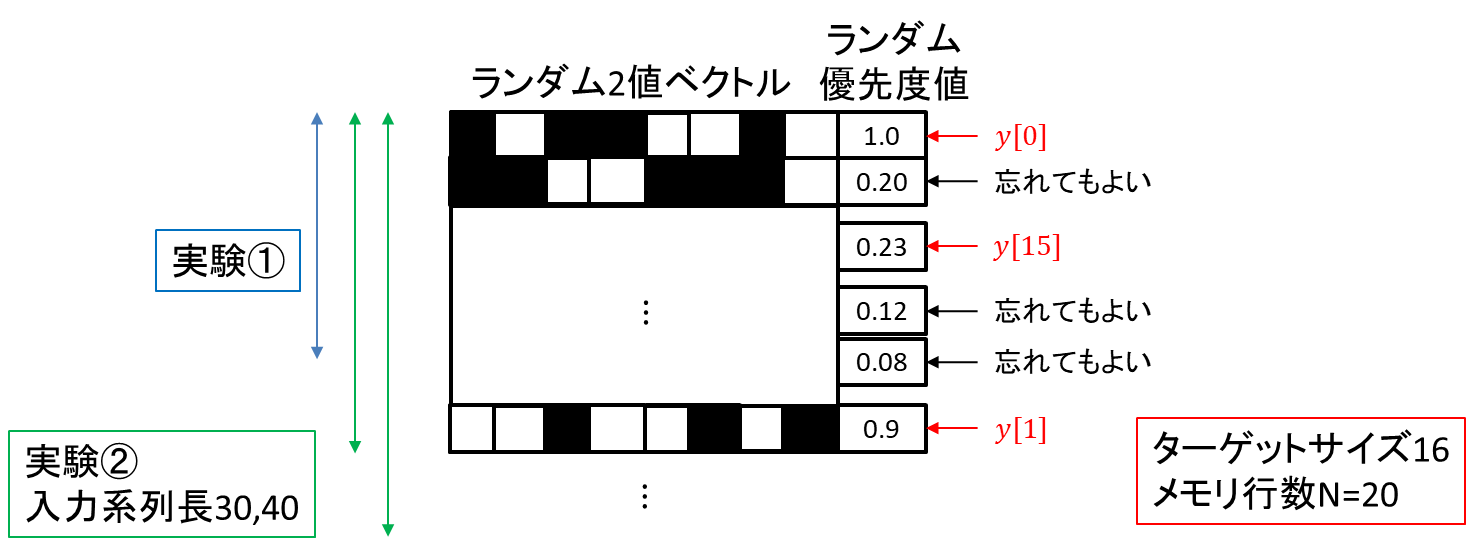
\includegraphics[width=\linewidth]{./figure/img_slide/priority.png}
	\caption{priority sort タスク}
	\label{fig:priority}
\end{figure}

\subsection{実験結果}
表\ref{table:result-1}に

\section{実験2 priority sortにおける長期入力系列の検証}
 4.2節のタスクにおいて入力系列のサイズを増加させたときの精度の推移を観察する。この実験により提案ネットワークが長期依存関係を扱う能力を評価する。
提案ネットワークは入力系列が長期にわたるとき、分散型項目メモリを持つSAMよりも正答率が高くなることが期待される。

\section{実験3 Nth-farthest}
この実験の目的は提案手法がNTMに関係推論能力を付与出来るかを評価することである。
既存研究\cite{rrnn}\cite{sam}はRMCやSTMのような関係推論能力を持つモデルが90以上の精度を記録した一方で、
NTMやDNCの精度は30を超えないことを示している。
提案ネットワークがNTMメモリ項目間の関係を計算できる場合、NTMよりも大きく改善された精度を示すことが期待される。

入力系列はランダムに生成されたバイナリベクトルからなる。ベクトルの次元を$d$、系列長を$l$で表したとき、タスクの要求は入力系列中のあるベクトル$m$から$n$番目に遠いベクトルを見つける事である。$m,n$は入力系列ごとにランダムに決定される。
1ステップあたりの入力はバイナリベクトル、ベクトルのID、$m$、$n$を連結したベクトルからなり、$ID,m,n∈\{1,2,…,l\}$はone-hotエンコーディングにより表現されるため、最終的な入力の次元は$d+3l$になる。
既存研究\cite{rrnn}に従い、$d=16,l=8$として実験を行った。

このタスクは入力の読み書きやソートといったタスクよりも複雑な処理をネットワークに要求する。
ネットワークは$m$と全入力のペアの距離を計算しソートを行う必要がある。距離は入力間の関係情報の一形態である。
入力そのものをソートするタスクと異なり、関係情報のソートの為に関係メモリを活用する必要がある。


\section{実験4 babi dataset}

\begin{comment}
	また,ああああああ
\end{comment}

\begin{table}[H]
	\caption{あああといいいの予測誤差}
	\centering
	\scalebox{0.98}[0.98]{
		\begin{tabular}{c|c|c|c|c|c|c}
			\multicolumn{1}{c}{} & \multicolumn{2}{|c|}{2019} 
			& \multicolumn{2}{c|}{2018} & \multicolumn{2}{c}{2017}\\ \hline \hline
			モデル    & ああ & いい & ああ & いい & ああ & いい \\ \hline
			Naive    & \bf{1} & 1 & \bf{1} & 1 & \bf{1} & 1 \\
			TCN      & 1.0895 & 0.9032 & 1.4791 & \bf{0.9198} & 1.2888 & 0.8555 \\
			LSTM     & 1.0384 & 0.9295 & 1.4917 & 0.9725 & 1.1627 & 0.8541 \\
			提案手法  & 1.0977 & \bf{0.8698} & 1.3824 & 0.9439 & 1.2061 & \bf{0.8516} \\
		\end{tabular}
	}
	\label{table:result-1}
\end{table}
